% presentaciones/sesion07-cap07/sesion07.tex
% Sesión 7 — Capítulo 7: Customer journey: del interés a la satisfacción y su mapeo
% Laboratorio: Gestión de datos, comportamiento y perfiles del consumidor digital
% Lic. en Mercadotecnia Digital · ESCA Unidad Santo Tomás · IPN
% Fuente de contenido: libro-consumidor-digital/partes/parte2/cap07.tex
% Figuras reutilizadas del libro (TikZ y MATLAB) sin copiarlas: ver \graphicspath y \input.
\documentclass[aspectratio=169,xcolor=dvipsnames]{beamer}
\usetheme{Berlin}

%----------------------------------------------------------------------------------------
%   PALETA INSTITUCIONAL IPN (Manual de Identidad Gráfica, Pantone 222C)
%----------------------------------------------------------------------------------------
\usepackage[dvipsnames,svgnames,x11names]{xcolor}
\definecolor{IPNguinda}{HTML}{6F1D46}       % Pantone 222C oficial — color primario
\definecolor{IPNguindaOsc}{HTML}{45102C}    % sombra / paleta secundaria
\definecolor{IPNguindaClara}{HTML}{F4E9EF}  % fondo de bloques normales
\definecolor{IPNdorado}{HTML}{B8975A}       % dorado — SOLO enlaces y detalles del cierre
\definecolor{IPNterracota}{HTML}{9C5B44}    % alertblock
\definecolor{IPNterracotaClara}{HTML}{F6ECE6}
\definecolor{IPNbronce}{HTML}{8C6B3F}       % exampleblock
\definecolor{IPNbronceClaro}{HTML}{F5F0E3}
\definecolor{IPNgris}{HTML}{58595B}         % texto secundario / notas

% Alias con los nombres de config/colores.tex del libro, para que las figuras
% TikZ del libro se puedan \input sin modificarlas
\colorlet{guindaIPN}{IPNguinda}
\colorlet{guindaIPNOsc}{IPNguindaOsc}
\colorlet{guindaIPNClara}{IPNguindaClara}
\colorlet{doradoIPN}{IPNdorado}
\colorlet{bronceIPN}{IPNbronce}
\colorlet{bronceIPNClaro}{IPNbronceClaro}
\colorlet{grisIPN}{IPNgris}
\colorlet{terracotaIPN}{IPNterracota}
\colorlet{terracotaIPNClara}{IPNterracotaClara}
\definecolor{colorLaboratorio}{HTML}{1B6E7A}

\setbeamercolor{palette primary}{bg=IPNguinda,fg=white}
\setbeamercolor{palette secondary}{bg=IPNguindaOsc,fg=white}
\setbeamercolor{palette tertiary}{bg=IPNguindaOsc,fg=white}
\setbeamercolor{palette quaternary}{bg=IPNguinda,fg=white}
\setbeamercolor{structure}{fg=IPNguinda}
\setbeamercolor{title}{bg=IPNguinda,fg=white}
\setbeamercolor{frametitle}{bg=IPNguinda,fg=white}
\setbeamercolor{block title}{bg=IPNguinda,fg=white}
\setbeamercolor{block body}{bg=IPNguindaClara,fg=black}
\setbeamercolor{block title alerted}{bg=IPNterracota,fg=white}
\setbeamercolor{block body alerted}{bg=IPNterracotaClara,fg=black}
\setbeamercolor{block title example}{bg=IPNbronce,fg=white}
\setbeamercolor{block body example}{bg=IPNbronceClaro,fg=black}
\setbeamercolor{alerted text}{fg=IPNterracota}
\setbeamercolor{item}{fg=IPNguinda}
\setbeamercolor{section in toc}{fg=IPNguinda}
\setbeamercolor{footline}{bg=IPNguindaOsc,fg=white}

\usepackage[spanish,es-noshorthands,es-nodecimaldot]{babel}
\usepackage{csquotes}
\usepackage{hyperref}
\usepackage{graphicx}
\usepackage{booktabs}
\usepackage{array}
\usepackage{amsmath}
\setbeamertemplate{caption}[numbered]
\usepackage{xurl}
\usepackage{adjustbox}
\usepackage{tikz}
\usetikzlibrary{arrows.meta,positioning}
\usepackage{pgfplots}
\pgfplotsset{compat=1.18}

\graphicspath{{Figures/}{../../libro-consumidor-digital/figuras/matlab/}}
\newcommand{\figtikz}[1]{../../libro-consumidor-digital/figuras/tikz/#1}
\newcommand{\fuente}[1]{{\tiny\color{IPNgris}Fuente: #1}}

\hypersetup{
    colorlinks=true,
    linkcolor=IPNdorado,
    filecolor=IPNguinda,
    urlcolor=IPNguinda,
    citecolor=IPNguinda,
    pdftitle={Sesion 7 - Customer journey},
    pdfauthor={Dr. Aboud Barsekh-Onji},
}

%----------------------------------------------------------------------------------------
%   CODE LISTINGS — sintaxis ESTÁNDAR del lenguaje
%----------------------------------------------------------------------------------------
\usepackage{listings}
\definecolor{backcolour}{rgb}{0.97,0.97,0.99}
\definecolor{codegreen}{rgb}{0,0.6,0}

\lstdefinestyle{MATLABStyle}{
  language=Matlab,
  basicstyle=\ttfamily\scriptsize,
  keywordstyle=\color{blue}\bfseries,
  commentstyle=\color{codegreen},
  stringstyle=\color{violet},
  breaklines=true,
  numbers=left,
  numbersep=5pt,
  frame=lines,
  backgroundcolor=\color{backcolour}
}
\lstset{style=MATLABStyle}

%----------------------------------------------------------------------------------------
%   TITLE CONFIGURATION
%----------------------------------------------------------------------------------------
\logo{
\includegraphics[height=0.75cm]{ipn-escudo.png}}
\title[Sesión 7 · Customer journey]{Customer journey: del interés a la satisfacción y su mapeo}
\subtitle{Sesión 7 · Unidad II — Capítulo 7}
\author{Dr. Aboud Barsekh-Onji}
\institute[IPN]{
    Instituto Politécnico Nacional \\
    \small ESCA Unidad Santo Tomás · Lic. en Mercadotecnia Digital \\
    \footnotesize Laboratorio: Gestión de datos, comportamiento y perfiles del consumidor digital
}
\date{\today}

%----------------------------------------------------------------------------------------
%   AUTO AGENDA AT EACH SECTION
%----------------------------------------------------------------------------------------
\AtBeginSection[]{
  \begin{frame}{Agenda}
    \tableofcontents[currentsection]
  \end{frame}
}



\begin{document}

\begin{frame}
    \titlepage
    \vspace{-4pt}
    \begin{center}
        {\tiny\color{IPNgris} ORCID: \href{https://orcid.org/0009-0004-5440-8092}{0009-0004-5440-8092}}
    \end{center}
\end{frame}

%------------------------------------------------
\section{Encuadre}
%------------------------------------------------

\begin{frame}{Ficha de la sesión}
\begin{columns}[T]
  \column{0.52\textwidth}
  \begin{block}{Unidad II}
    \small Proceso de toma de decisión de compra digital
  \end{block}
  \begin{block}{Tema del programa (2.2 \textit{Customer journey})}
    \scriptsize
    \begin{itemize}
      \item[2.2.1] Atención \quad [2.2.2] Interés \quad [2.2.3] Deseo
      \item[2.2.4] Acción \quad [2.2.5] Satisfacción
      \item[2.2.6] Mapeo del \textit{customer journey}
    \end{itemize}
  \end{block}
  \column{0.44\textwidth}
  \begin{block}{Carga horaria}
    \small Teoría 3.0 h · Práctica 2.0 h\\ Aprendizaje autónomo 1.0 h
  \end{block}
  \begin{exampleblock}{Competencia de la unidad}
    \small Examina el proceso de toma de decisiones de compra del consumidor digital a partir de su recorrido y figuras participantes.
  \end{exampleblock}
\end{columns}
\end{frame}

\begin{frame}{Al terminar la sesión podrás\ldots}
\begin{enumerate}
  \item \textbf{Recorrer} las cinco etapas AIDAS y traducirlas a puntos de contacto, datos y métricas.
  \vspace{4pt}
  \item \textbf{Explicar} por qué el embudo lineal describe mal la conducta y distinguir evidencia independiente de marcos de consultoría.
  \vspace{4pt}
  \item \textbf{Construir} un mapa de recorrido y declarar sus límites.
  \vspace{4pt}
  \item \textbf{Modelar} el recorrido como cadena de Markov y comparar tres modelos de atribución.
\end{enumerate}
\vspace{6pt}
\begin{alertblock}{Recordatorio}
  Aprendizaje autónomo de la Sesión 6: entrega en la fecha acordada en clase, en su carpeta del portafolio.
\end{alertblock}
\end{frame}

\begin{frame}{Arranque: ¿quién te convenció de comprar?}
\begin{columns}[T]
  \column{0.55\textwidth}
  \begin{exampleblock}{Pregunta de arranque}
    Piensen en la \textbf{última compra relevante} que hicieron en línea. ¿Qué fue lo \textbf{último} que vieron antes de pagar? ¿Y lo \textbf{primero} que supieron del producto?\\[4pt]
    ¿Fue el mismo canal?
  \end{exampleblock}
  \vspace{4pt}
  {\small\color{IPNgris} Puente con la Sesión 6: el caso real que eligió cada equipo.}
  \column{0.41\textwidth}
  \begin{block}{Dinámica (10 min)}
    \small
    \begin{enumerate}
      \item Individual: anoten primer y último contacto (2 min).
      \item Parejas: ¿qué hubo en medio?
      \item Pizarrón: ¿coinciden alguna vez el primero y el último?
    \end{enumerate}
  \end{block}
\end{columns}
\end{frame}

%------------------------------------------------
\section[Apertura]{Caso de apertura}
%------------------------------------------------

\begin{frame}{El modelo más citado no tiene inventor claro}
\begin{columns}[T]
  \column{0.48\textwidth}
  \begin{block}{La versión de los manuales}
    \small \textbf{E. St. Elmo Lewis, 1898}: atención, interés, deseo, acción. La atribución circula desde \textbf{1925} (Strong) y se repitió un siglo \textbf{sin consultar los documentos}.
  \end{block}
  \column{0.48\textwidth}
  \begin{alertblock}{Lo que encontró Iwamoto (2024)}
    \small Sin evidencia primaria de que Lewis lo formulara. \textbf{Sheldon y Dukesmith} lo teorizaron antes. El \textbf{acrónimo AIDA} es de \textbf{C. P. Russell, 1921} (\textit{Printers' Ink}).
  \end{alertblock}
\end{columns}
\vspace{6pt}
\begin{exampleblock}{Dos lecciones}
  \small Un modelo puede ser útil y su genealogía, dudosa. Y una narrativa repetida un siglo \textbf{no es evidencia}: vale igual para los marcos modernos de consultoras y plataformas.
\end{exampleblock}
\end{frame}

%------------------------------------------------
\section[AIDAS]{2.2.1--2.2.5 Las cinco etapas}
%------------------------------------------------

\begin{frame}{De AIDA a AIDAS}
\begin{columns}[T]
  \column{0.52\textwidth}
  \begin{block}{Qué es el \textit{customer journey}}
    \small El camino de una persona desde que se entera de una oferta hasta que la usa y opina sobre ella.
  \end{block}
  \begin{exampleblock}{Cinco etapas}
    \small \textbf{A}tención · \textbf{I}nterés · \textbf{D}eseo · \textbf{A}cción · \textbf{S}atisfacción
  \end{exampleblock}
  \column{0.44\textwidth}
  \begin{alertblock}{Cuidado}
    \scriptsize AIDA nació para la venta personal y la publicidad impresa. Su lectura digital es una \textbf{reinterpretación aplicada}, no una cita de Sheldon, Lewis ni Strong. La \textbf{S} es una extensión posterior: conecta con la etapa 2.1.5.
  \end{alertblock}
\end{columns}
\end{frame}

\begin{frame}{Lectura digital de cada etapa}
\footnotesize
\begin{center}
\begin{tabular}{@{}>{\raggedright}p{1.9cm}>{\raggedright}p{3.2cm}>{\raggedright}p{3.0cm}>{\raggedright\arraybackslash}p{2.7cm}@{}}
\toprule
\textbf{Etapa} & \textbf{Punto de contacto} & \textbf{Dato que deja} & \textbf{Métrica} \\
\midrule
Atención & Anuncio, publicación, resultado de búsqueda & Impresión, tiempo de visualización & Alcance, frecuencia \\
Interés & Visita al sitio, reseñas & Clic, tiempo en página & Tasa de clics \\
Deseo & Guardar, comparar, carrito & Evento \enquote{agregar al carrito} & Abandono de carrito \\
Acción & \textit{Checkout} y pago & Transacción & Tasa de conversión \\
Satisfacción & Entrega, soporte, reseña & Calificación, devolución & Recompra, recomendación \\
\bottomrule
\end{tabular}
\end{center}
\fuente{elaboración propia. Reinterpretación aplicada, no formulación original.}
\end{frame}

\begin{frame}{Tres advertencias por etapa}
\begin{columns}[T]
  \column{0.31\textwidth}
  \begin{alertblock}{Atención}
    \small \textbf{Exposición no es atención}: un anuncio puede cargar sin que nadie lo vea. La impresión es una oportunidad, no un hecho psicológico.
  \end{alertblock}
  \column{0.31\textwidth}
  \begin{block}{Deseo}
    \small Es la etapa más difícil de observar: ocurre \textbf{dentro} de la persona. Los datos capturan solo su sombra (producto guardado, carrito sin pagar).
  \end{block}
  \column{0.31\textwidth}
  \begin{exampleblock}{Acción}
    \small Es la que mejor se mide y por eso \textbf{se sobrevalora}: se atribuye todo a lo que pasó justo antes del pago.
  \end{exampleblock}
\end{columns}
\vspace{6pt}
{\small\color{IPNgris} El laboratorio de hoy cuantifica cuánto distorsiona esa costumbre.}
\end{frame}

\begin{frame}{Un marco contemporáneo: las 5A de Kotler}
\begin{columns}[T]
  \column{0.55\textwidth}
  \begin{block}{\textit{Aware} · \textit{Appeal} · \textit{Ask} · \textit{Act} · \textit{Advocate}}
    \small Conocer, atraer, preguntar, actuar, recomendar. Añade dos ideas útiles: \textbf{preguntar} (consultar a pares y a la marca) y \textbf{recomendar} (la satisfacción se vuelve influencia).
  \end{block}
  \column{0.41\textwidth}
  \begin{alertblock}{Cómo leerlo}
    \small Propuesta de consultoría y libro de texto (Kotler et al., 2021): \textbf{valor pedagógico}, sin validación empírica independiente.
  \end{alertblock}
\end{columns}
\end{frame}

%------------------------------------------------
\section[Embudo y bucle]{Frontera: del embudo al bucle}
%------------------------------------------------

\begin{frame}{El embudo lineal describe mal lo que la gente hace}
\begin{center}
  \adjustbox{max width=0.9\linewidth,max height=0.55\textheight}{\input{\figtikz{cap07-embudo-vs-bucle}}}
\end{center}
\vspace{2pt}
\begin{itemize}
  \small
  \item El embudo sigue siendo un buen \textbf{punto de partida pedagógico}.
  \item Pero las personas \textbf{exploran y evalúan varias veces}, agregan y quitan marcas y regresan.
\end{itemize}
\fuente{elaboración propia, a partir de Court et al. (2009) y Think with Google (2020).}
\end{frame}

\begin{frame}{Qué respaldo tiene cada marco}
\scriptsize
\begin{center}
\begin{tabular}{@{}>{\raggedright}p{2.2cm}>{\raggedright}p{2.7cm}>{\raggedright}p{3.2cm}>{\raggedright\arraybackslash}p{2.6cm}@{}}
\toprule
\textbf{Marco} & \textbf{Origen} & \textbf{Evidencia} & \textbf{Cuidado} \\
\midrule
AIDA / AIDAS & Venta y publicidad de inicios del s. XX & Modelo conceptual sin prueba empírica original & No es una descripción verificada \\
\textit{Consumer decision journey} & Consultora (Court et al., 2009) & ${\sim}$20\,000 consumidores, 5 industrias, 3 países; no arbitrado & Investigación de una consultora \\
\textit{Messy middle} & Plataforma publicitaria (2020) & 310\,000 escenarios simulados & Conflicto de interés declarado \\
5A & Consultoría (Kotler et al., 2021) & Propuesta sin validación independiente & Marco pedagógico \\
\bottomrule
\end{tabular}
\end{center}
\vspace{2pt}
\begin{alertblock}{La distinción que importa}
  \scriptsize La crítica al embudo lineal \textbf{sí} tiene respaldo académico independiente (Santos y Gonçalves, 2021, revista arbitrada). Los modelos de marca son \textbf{marcos útiles con estudio propio}, no experimentos neutrales.
\end{alertblock}
\fuente{elaboración propia.}
\end{frame}

\begin{frame}{Y en 2026: asistentes de compra con IA}
\begin{columns}[T]
  \column{0.52\textwidth}
  \begin{block}{Qué cambia}
    \small Los asistentes pueden \textbf{absorber parte de la exploración y la evaluación}. El tramo caótico se comprime en una conversación.
  \end{block}
  \column{0.44\textwidth}
  \begin{alertblock}{La pregunta de fondo no cambia}
    \small ¿\textbf{Quién reduce las opciones} antes de la decisión final? Ya la vimos con el comercio agéntico (Sesión 4).
  \end{alertblock}
\end{columns}
\end{frame}

%------------------------------------------------
\section[Mapeo]{2.2.6 Mapeo del recorrido}
%------------------------------------------------

\begin{frame}{Un mapa de recorrido (caso ilustrativo)}
\begin{center}
  \adjustbox{max width=0.97\linewidth,max height=0.72\textheight}{\input{\figtikz{cap07-mapa-journey}}}
\end{center}
\fuente{elaboración propia. Caso ficticio.}
\end{frame}

\begin{frame}{Para qué sirve un mapa y qué no promete}
\begin{columns}[T]
  \column{0.48\textwidth}
  \begin{exampleblock}{Sirve para forzar preguntas}
    \small ¿Qué \textbf{dato} tengo en cada etapa? ¿Dónde se \textbf{enfría la emoción}? ¿Qué canal es \textbf{de otro}? Lemon y Verhoef (2016) clasifican los puntos de contacto: de la marca, de socios, del cliente y sociales.
  \end{exampleblock}
  \column{0.48\textwidth}
  \begin{alertblock}{No es un registro del camino real}
    \small La promesa de un recorrido \enquote{a 360 grados} no tiene respaldo académico. Dispositivos e identidades fragmentados, \textit{cookies} bloqueadas y asistentes de IA van en sentido contrario. Un mapa \textbf{ordena la conversación}; no registra la realidad.
  \end{alertblock}
\end{columns}
\end{frame}

%------------------------------------------------
\section[Evidencia]{Evidencia: México}
%------------------------------------------------

\begin{frame}{El recorrido ocurre en varios lugares a la vez}
\begin{columns}[T]
  \column{0.52\textwidth}
  \begin{block}{México, 2025}
    \small
    \begin{itemize}
      \item \textbf{86.1\,\%} de la población de 6 años o más usó internet (104.9 millones de personas). INEGI (2026).
      \item El comercio electrónico minorista fue \textbf{17.7\,\%} de las ventas del sector. AMVO (2026).
    \end{itemize}
  \end{block}
  \column{0.44\textwidth}
  \begin{alertblock}{Implicación metodológica}
    \small Mucha gente \textbf{recorre etapas en línea y compra en tienda}. Un mapa hecho solo con datos de la tienda en línea ve un \textbf{fragmento} del recorrido.
  \end{alertblock}
\end{columns}
\fuente{INEGI (2026); Asociación Mexicana de Venta Online (2026). Fuentes distintas: no se suman.}
\end{frame}

%------------------------------------------------
\section[Laboratorio]{Laboratorio MATLAB}
%------------------------------------------------

\begin{frame}{Laboratorio: el recorrido como cadena de Markov}
\begin{block}{Objetivo}
  Modelar las etapas con dos estados absorbentes (Conversión y Abandono), calcular probabilidad y tiempo de conversión, compararlos con un embudo lineal y atribuir las conversiones entre cuatro canales con tres modelos.
\end{block}
\begin{columns}[T]
  \column{0.52\textwidth}
  \begin{exampleblock}{Cadena de Markov}
    \scriptsize
    El siguiente paso depende solo del estado actual.
    \[ N=(I-Q)^{-1},\quad B=NR,\quad \mathbb{E}[T]=N\mathbf{1} \]
    $Q$: transiciones entre etapas. $R$: hacia Conversión/Abandono.
  \end{exampleblock}
  \column{0.44\textwidth}
  \begin{block}{Tres modelos de atribución}
    \scriptsize
    \textbf{Último clic:} todo al canal final. \textbf{Primer clic:} todo al inicial. \textbf{Efecto de remoción:} cuánto cae la probabilidad de convertir si se quita el canal (Anderl et al., 2016).
  \end{block}
\end{columns}
\end{frame}

\begin{frame}[fragile]{El script: \texttt{cap07\_journey\_markov.m}}
\begin{columns}[T]
  \column{0.62\textwidth}
\begin{lstlisting}[basicstyle=\ttfamily\tiny]
%% ==================================
%  PARAMETROS: UNICA SECCION QUE
%  EL ESTUDIANTE DEBE EDITAR
%  ==================================
pAvanzar = 0.30;     % siguiente etapa (> 0)
pRetroceder = 0.10;  % vuelve a la anterior
pAbandonar = 0.15;   % sale del recorrido
inicioRedes = 0.40;  % % que empieza en redes
convBusqueda = 0.30; % convierte desde busqueda
convDirecto = 0.35;  % convierte desde directo
\end{lstlisting}
  \column{0.34\textwidth}
  \begin{block}{Reglas y rangos}
    \scriptsize
    \begin{itemize}
      \item \texttt{pAvanzar} $>0$; la suma de las tres primeras $\le 1$.
      \item \texttt{inicioRedes} entre 0 y 1; \texttt{convBusqueda} hasta 0.60; \texttt{convDirecto} hasta 0.80.
      \item Datos \textbf{sintéticos}; sin azar: cálculo exacto.
    \end{itemize}
  \end{block}
  \begin{exampleblock}{Sin MATLAB}
    \scriptsize \texttt{cap07\_journey\_markov\_\allowbreak interactivo.html}: mismos parámetros y casos A, B, C.
  \end{exampleblock}
\end{columns}
\end{frame}

\begin{frame}{Salida: matriz de transición y tiempo a conversión}
\begin{center}
  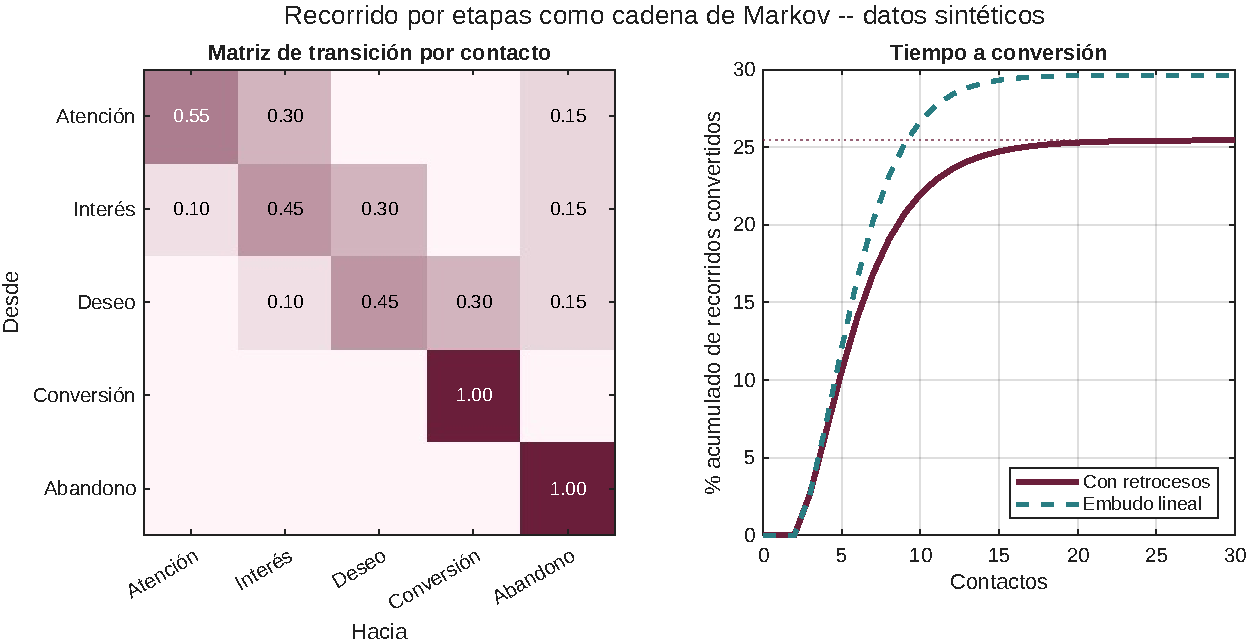
\includegraphics[width=\linewidth,height=0.62\textheight,keepaspectratio]{cap07_markov_etapas.pdf}
\end{center}
\vspace{-4pt}
\begin{center}
  \small Convierte \textbf{25.4\,\%} (embudo lineal: 29.6\,\%) · convertidos en 10 contactos o menos: \textbf{22.0\,\%} (lineal: 26.7\,\%)
\end{center}
\fuente{elaboración propia, MATLAB, datos sintéticos.}
\end{frame}

\begin{frame}{Interpretación: el costo de volver atrás}
\begin{columns}[c]
  \column{0.48\textwidth}
  \begin{block}{Lo que muestran las curvas}
    \small Volver atrás \textbf{baja la conversión} y \textbf{la retrasa}: 6.95 contactos hasta convertir contra 6.67 en el embudo lineal.
  \end{block}
  \begin{alertblock}{El error costoso}
    \small Un embudo lineal que ignora los retrocesos \textbf{sobreestima} cuántos convierten y \textbf{subestima} cuánto tardan.
  \end{alertblock}
  \column{0.48\textwidth}
  \begin{exampleblock}{Mensaje para la marca}
    \small Cada contacto en que la persona regresa a evaluar es una oportunidad de dar \textbf{información clara}, no de empujar con urgencia falsa (Sesión 6).
  \end{exampleblock}
\end{columns}
\end{frame}

\begin{frame}{Salida: ¿qué canal se lleva el crédito?}
\begin{center}
  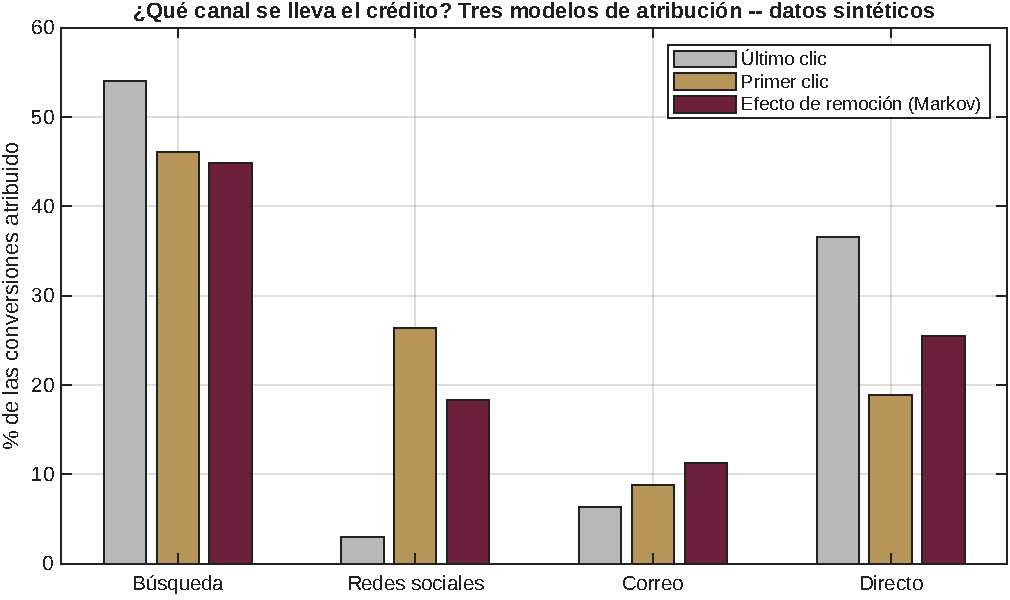
\includegraphics[width=\linewidth,height=0.62\textheight,keepaspectratio]{cap07_atribucion.pdf}
\end{center}
\vspace{-4pt}
\begin{center}
  \small \textbf{Redes sociales:} 3.0\,\% con el último clic, \textbf{18.3\,\%} con el efecto de remoción.
\end{center}
\fuente{elaboración propia, MATLAB, datos sintéticos.}
\end{frame}

\begin{frame}{Interpretación: quien abre no cierra}
\begin{columns}[c]
  \column{0.48\textwidth}
  \begin{block}{Lo que pasa}
    \small Redes sociales casi nunca es el último contacto: \textbf{abre recorridos y los pasa a búsqueda}.
  \end{block}
  \begin{alertblock}{La decisión equivocada}
    \small Presupuestar con el último clic recorta \textbf{el canal que alimenta a los demás}.
  \end{alertblock}
  \column{0.48\textwidth}
  \begin{exampleblock}{Versión cuantitativa de una advertencia}
    \small La \textbf{acción} es la etapa mejor medida y por eso la más sobrevalorada. Un modelo puede ser correcto en sus cálculos y engañoso en su uso.
  \end{exampleblock}
\end{columns}
\end{frame}

\begin{frame}{Ejercicio propuesto: tres corridas}
\begin{columns}[T]
  \column{0.52\textwidth}
  \begin{exampleblock}{Casos (solo el bloque de parámetros)}
    \scriptsize
    \begin{itemize}
      \item[\textbf{A}] Valores por defecto.
      \item[\textbf{B}] \textbf{Recorrido desordenado}: \texttt{pRetroceder} de 0.10 a 0.25.
      \item[\textbf{C}] \textbf{Más redes y mejor directo}: \texttt{pRetroceder} en 0.10, \texttt{inicioRedes} = 0.70 y \texttt{convDirecto} = 0.60.
    \end{itemize}
  \end{exampleblock}
  \column{0.44\textwidth}
  \scriptsize
  \begin{tabular}{@{}lcccc@{}}
    \toprule
    Caso & \% conv. & Contact. & UC & Rem. \\
    \midrule
    A & \rule{0.55cm}{0.4pt} & \rule{0.55cm}{0.4pt} & \rule{0.55cm}{0.4pt} & \rule{0.55cm}{0.4pt} \\[2pt]
    B & \rule{0.55cm}{0.4pt} & \rule{0.55cm}{0.4pt} & \rule{0.55cm}{0.4pt} & \rule{0.55cm}{0.4pt} \\[2pt]
    C & \rule{0.55cm}{0.4pt} & \rule{0.55cm}{0.4pt} & \rule{0.55cm}{0.4pt} & \rule{0.55cm}{0.4pt} \\
    \bottomrule
  \end{tabular}\\[2pt]
  {\tiny Contact.: contactos hasta convertir. UC / Rem.: \% de crédito de Redes con último clic / remoción.}
\end{columns}
\vspace{2pt}
\begin{block}{Respondan con sus corridas}
  \scriptsize
  \begin{enumerate}
    \item Caso B: ¿qué pasa con la conversión y el tiempo? ¿Qué le dice a una marca que mide su embudo como si fuera lineal?
    \item Caso C: ¿cambia el crédito de Redes con el último clic? ¿Y con la remoción?
    \item ¿Por qué un modelo de atribución puede engañar aunque sus cálculos sean correctos?
  \end{enumerate}
\end{block}
\end{frame}

\begin{frame}{Segundo insumo de la práctica «Recorrido del consumidor digital»}
\begin{columns}[T]
  \column{0.54\textwidth}
  \begin{block}{Sobre el caso que eligieron en la Sesión 6}
    \small Hoy agregan al entregable único el \textbf{recorrido AIDAS} de su caso y un \textbf{mapa} con punto de contacto, emoción, dato que deja y oportunidad o dolor por etapa.
  \end{block}
  \column{0.42\textwidth}
  \begin{exampleblock}{Wiki de mapeo}
    \scriptsize
    \begin{itemize}
      \item Suban el mapa del equipo a la wiki del grupo.
      \item Comenten el mapa de \textbf{otro equipo}: ¿qué dato falta? ¿qué canal es de otro?
    \end{itemize}
  \end{exampleblock}
\end{columns}
\end{frame}

\begin{frame}{Práctica con sus propios datos: app HTML}
\begin{columns}[T]
  \column{0.54\textwidth}
  \begin{block}{\texttt{cap07\_journey\_datos\_propios.html}}
    \small Sin MATLAB y sin conexión: suban un Excel con \textbf{sus datos} y recorran 5 pasos:
    \scriptsize
    \begin{enumerate}
      \item Sus recorridos y las rutas más frecuentes.
      \item La cadena de Markov que sus datos estiman.
      \item Cuatro modelos de atribución.
      \item ¿Qué pasa si se apaga un canal?
      \item Lectura de negocio y descarga en Excel.
    \end{enumerate}
  \end{block}
  \column{0.42\textwidth}
  \begin{exampleblock}{Reglas del archivo}
    \scriptsize
    \begin{itemize}
      \item Hoja \texttt{Recorridos}: \texttt{Canales} (A>B>C) y \texttt{Convirtio} (1/0 o Sí/No).
      \item Opcional: \texttt{Cantidad} para rutas agrupadas.
      \item \textbf{Sin} identificadores personales: el ID es un consecutivo.
      \item Sus datos \textbf{no salen} de su computadora.
    \end{itemize}
  \end{exampleblock}
\end{columns}
\end{frame}

\begin{frame}{Ética: unir rastros reduce el anonimato}
\begin{alertblock}{Reconstruir el recorrido de una persona exige juntar sus rastros}
  Lo que vio en una red social, lo que buscó, lo que abrió en el correo, lo que compró. \textbf{Cada unión reduce su anonimato.}
\end{alertblock}
\begin{block}{Como mínimo}
  \begin{itemize}
    \item El modelo del laboratorio trabaja con recorridos \textbf{agregados}; un mapa individual no.
    \item Antes de cruzar fuentes: ¿la \textbf{finalidad} lo justifica? ¿hay \textbf{base legal} para cada fuente (Sesión 3)? ¿bastarían datos agregados?
    \item Presentar como \enquote{recorrido completo} lo que es una muestra estilizada \textbf{induce a decidir con certeza que no existe}.
  \end{itemize}
\end{block}
\end{frame}

%------------------------------------------------
\section[Caso]{Estudio de caso}
%------------------------------------------------

\begin{frame}{Caso: la marca de ropa deportiva}
\begin{exampleblock}{Caso ficticio}
  Una marca mexicana vende en línea. Su informe de \textbf{último clic} dice: redes sociales \textbf{3\,\%}, búsqueda \textbf{54\,\%}, directo \textbf{37\,\%}. La dirección \textbf{pasa el presupuesto de redes a búsqueda de pago}.
\end{exampleblock}
\begin{alertblock}{Tres meses después}
  Las ventas totales \textbf{bajan} y el costo por clic de búsqueda \textbf{sube}. Un analista reconstruye los recorridos con una cadena de Markov: apagar redes sociales haría caer la probabilidad global de convertir \textbf{cerca de una quinta parte}.
\end{alertblock}
\end{frame}

\begin{frame}{Preguntas guía}
\small
\begin{enumerate}
  \item ¿Por qué el último clic casi no acredita a redes sociales? ¿Qué \textbf{papel} juega el canal en el recorrido?
  \vspace{3pt}
  \item Expliquen con el lenguaje de la sesión por qué \textbf{las ventas bajaron} y \textbf{el costo de búsqueda subió}.
  \vspace{3pt}
  \item Señalen una \textbf{limitación} del efecto de remoción como medida de causa. ¿Qué experimento diseñarían para confirmarlo?
  \vspace{3pt}
  \item ¿Qué \textbf{datos de identidad} necesitaría cruzar el analista y qué obligaciones legales implican?
\end{enumerate}
\begin{alertblock}{Entregable}
  \small Solución escrita con las cuatro preguntas respondidas.
\end{alertblock}
\end{frame}

%------------------------------------------------
\section{Cierre}
%------------------------------------------------

\begin{frame}{Síntesis: un recorrido que se mapea, no que se registra}
\begin{itemize}
  \small
  \item Cinco etapas: \textbf{atención, interés, deseo, acción y satisfacción}, traducidas a puntos de contacto, datos y métricas.
  \item AIDA tiene una \textbf{genealogía débil}; los marcos que la sustituyen son de consultoras y plataformas. La crítica al embudo lineal \textbf{sí} tiene respaldo independiente.
  \item Un mapa de recorrido es una \textbf{representación estilizada}: ordena la conversación, no registra el camino real.
  \item Con Markov se cuantifica el \textbf{costo de los retrocesos} y se reparte el crédito de las conversiones mejor que con el último clic.
\end{itemize}
\vspace{4pt}
\begin{alertblock}{La regla de la sesión}
  \small Antes de recortar un canal, pregunten: \textbf{¿qué recorridos dejarían de empezar si lo apago?}
\end{alertblock}
\end{frame}

\begin{frame}{Autoevaluación rápida}
\footnotesize
\begin{enumerate}
  \item La atribución de AIDA a Lewis (1898):
  \begin{itemize}
    \item[a)] está plenamente documentada con fuentes primarias;
    \item[b)] \alt<2->{\textcolor{IPNguinda}{\textbf{se apoya en una fuente secundaria de 1925 y carece de evidencia primaria}}}{se apoya en una fuente secundaria de 1925 y carece de evidencia primaria};
    \item[c)] nunca ha sido discutida.
  \end{itemize}
  \item La crítica al embudo lineal:
  \begin{itemize}
    \item[a)] solo la sostiene Google con su estudio propietario;
    \item[b)] \alt<2->{\textcolor{IPNguinda}{\textbf{tiene respaldo académico independiente, aunque los modelos de marca sean de consultoras o plataformas}}}{tiene respaldo académico independiente, aunque los modelos de marca sean de consultoras o plataformas};
    \item[c)] no tiene respaldo empírico.
  \end{itemize}
  \item El efecto de remoción de un canal mide:
  \begin{itemize}
    \item[a)] la proporción de recorridos que terminan en él;
    \item[b)] \alt<2->{\textcolor{IPNguinda}{\textbf{la caída de la probabilidad de convertir si se elimina ese canal}}}{la caída de la probabilidad de convertir si se elimina ese canal};
    \item[c)] su costo por clic.
  \end{itemize}
\end{enumerate}
\end{frame}


\begin{frame}{Evidencias del portafolio}
\begin{block}{Pasos para subir los trabajos al portafolio}
    \begin{itemize}
    \item Accede a esta carpeta de evidencia: \url{https://drive.google.com/drive/folders/1sr_SAVkl_Mjil6ZRWz3O2mveMoZVW6cp?usp=sharing}
    \item Crea una carpeta con tu nombre y organiza en ella todos tus entregables del semestre.
    \item Considera los tiempos límite establecidos para cada actividad.
    \end{itemize}
  \end{block}
\end{frame}


\begin{frame}{Evidencias del portafolio}
\small
\begin{columns}[T]
  \column{0.48\textwidth}
  \begin{block}{Infografía colaborativa}
    \scriptsize \textit{Customer journey} del caso real: cinco etapas AIDAS, puntos de contacto y métricas de cada una.
  \end{block}
  \begin{block}{Participación en wiki de mapeo}
    \scriptsize Mapa del caso (emoción, dato que deja, oportunidad o dolor) y comentario al mapa de otro equipo.
  \end{block}
  \column{0.48\textwidth}
  \begin{block}{Solución de casos}
    \scriptsize Caso de la marca de ropa deportiva, cuatro preguntas por escrito.
  \end{block}
  \begin{block}{Reporte de práctica}
    \scriptsize Cuadro de los casos A, B y C con las respuestas. Se integra al entregable único de «Recorrido del consumidor digital».
  \end{block}
\end{columns}
\end{frame}

\begin{frame}{Aprendizaje autónomo}
\footnotesize
\begin{enumerate}
  \item Ejecutar \texttt{cap07\_journey\_markov\_\allowbreak interactivo.html}, completar el cuadro de los \textbf{casos A, B y C} y anotar qué parámetro más cambia el crédito de Redes sociales.
  \vspace{1pt}
  \item Marcar en el mapa del caso del equipo cada punto de contacto como \textbf{de la marca, de socios, del cliente o social/externo}.
  \vspace{1pt}
  \item Elegir uno de los marcos del cuadro de respaldo y redactar \textbf{media cuartilla} sobre quién lo produjo y qué intereses tenía.
  \vspace{1pt}
  \item (Opcional) Con \texttt{cap07\_journey\_datos\_propios.html} (opcional), cargar el \textbf{Ejemplo 2} (tienda de ropa) y escribir en dos líneas qué canal se subestima con el último clic.
\end{enumerate}
\vspace{2pt}
\begin{alertblock}{Fecha de entrega}
  En la fecha acordada en clase, en su carpeta del portafolio.
\end{alertblock}
\end{frame}

\begin{frame}{Glosario de la sesión}
\scriptsize
\begin{description}
  \item[AIDAS] Atención, interés, deseo, acción y satisfacción.
  \item[Cadena de Markov] Proceso en que el siguiente estado depende solo del actual.
  \item[Estado absorbente] Del que no se sale: Conversión o Abandono.
  \item[\textit{Messy middle}] Ir y venir entre explorar y evaluar entre el disparador y la compra.
  \item[Último / primer clic] Todo el crédito al último / primer canal del recorrido.
  \item[Efecto de remoción] Caída de la probabilidad de convertir al eliminar un canal.
  \item[Probabilidad de retroceder] \texttt{pRetroceder}: real entre 0 y 1 (0 = embudo lineal); casos didácticos 0.10 y 0.25.
\end{description}
\end{frame}

\begin{frame}{Referencias}
\tiny
\begin{itemize}
  \item[] Anderl, E., Becker, I., von Wangenheim, F. y Schumann, J. H. (2016). Mapping the customer journey: Lessons learned from graph-based online attribution modeling. \textit{International Journal of Research in Marketing, 33}(3), 457--474. \url{https://doi.org/10.1016/j.ijresmar.2016.03.001}
  \item[] Asociación Mexicana de Venta Online. (2026). \textit{Estudio de Venta Online 2026}. AMVO.
  \item[] Court, D., Elzinga, D., Mulder, S. y Vetvik, O. J. (2009). The consumer decision journey. \textit{McKinsey Quarterly}, junio.
  \item[] Instituto Nacional de Estadística y Geografía. (2026). \textit{ENDUTIH 2025} (Comunicado de prensa 32/26). INEGI.
  \item[] Iwamoto, A. (2024). The origin of AIDA: Who invented and formulated the AIDA model? \textit{Japan Marketing History Review, 3}(2), 150--166.
  \item[] Kotler, P., Kartajaya, H. y Setiawan, I. (2021). \textit{Marketing 5.0: Technology for humanity}. Wiley.
  \item[] Lemon, K. N. y Verhoef, P. C. (2016). Understanding customer experience throughout the customer journey. \textit{Journal of Marketing, 80}(6), 69--96. \url{https://doi.org/10.1509/jm.15.0420}
  \item[] Santos, S. y Gonçalves, H. M. (2021). The consumer decision journey: A literature review of the foundational models and theories and a future perspective. \textit{Technological Forecasting and Social Change, 173}, 121117. \url{https://doi.org/10.1016/j.techfore.2021.121117}
  \item[] Think with Google. (2020). \textit{Decoding decisions: The messy middle of purchase behavior}. Google.
\end{itemize}
\end{frame}

\begin{frame}
    \begin{center}
        {\Large \textcolor{IPNguinda}{\textbf{Gracias}}}\\[6pt]
        {\color{IPNdorado}\rule{0.4\linewidth}{1.2pt}}\\[6pt]
        Dr. Aboud Barsekh-Onji \\
        \small Instituto Politécnico Nacional · ESCA Unidad Santo Tomás \\
        \small \texttt{ORCID: \href{https://orcid.org/0009-0004-5440-8092}{0009-0004-5440-8092}}
    \end{center}
\end{frame}

\end{document}
